\begin{lstlisting}[language=alloy]
    
    run VisitorEntersTheStoreAtTheStore for 5 but 3 Time
    run CustomerEntersTheStore for 5 but 3 Time
    run CustomerEntersTheStoreQRCode for 5 but 3 Time
    run CustomerEntersTheStoreVisit for 5 but 2 Time

\end{lstlisting}

\subsection{Proof of consistency}

    \begin{center}
        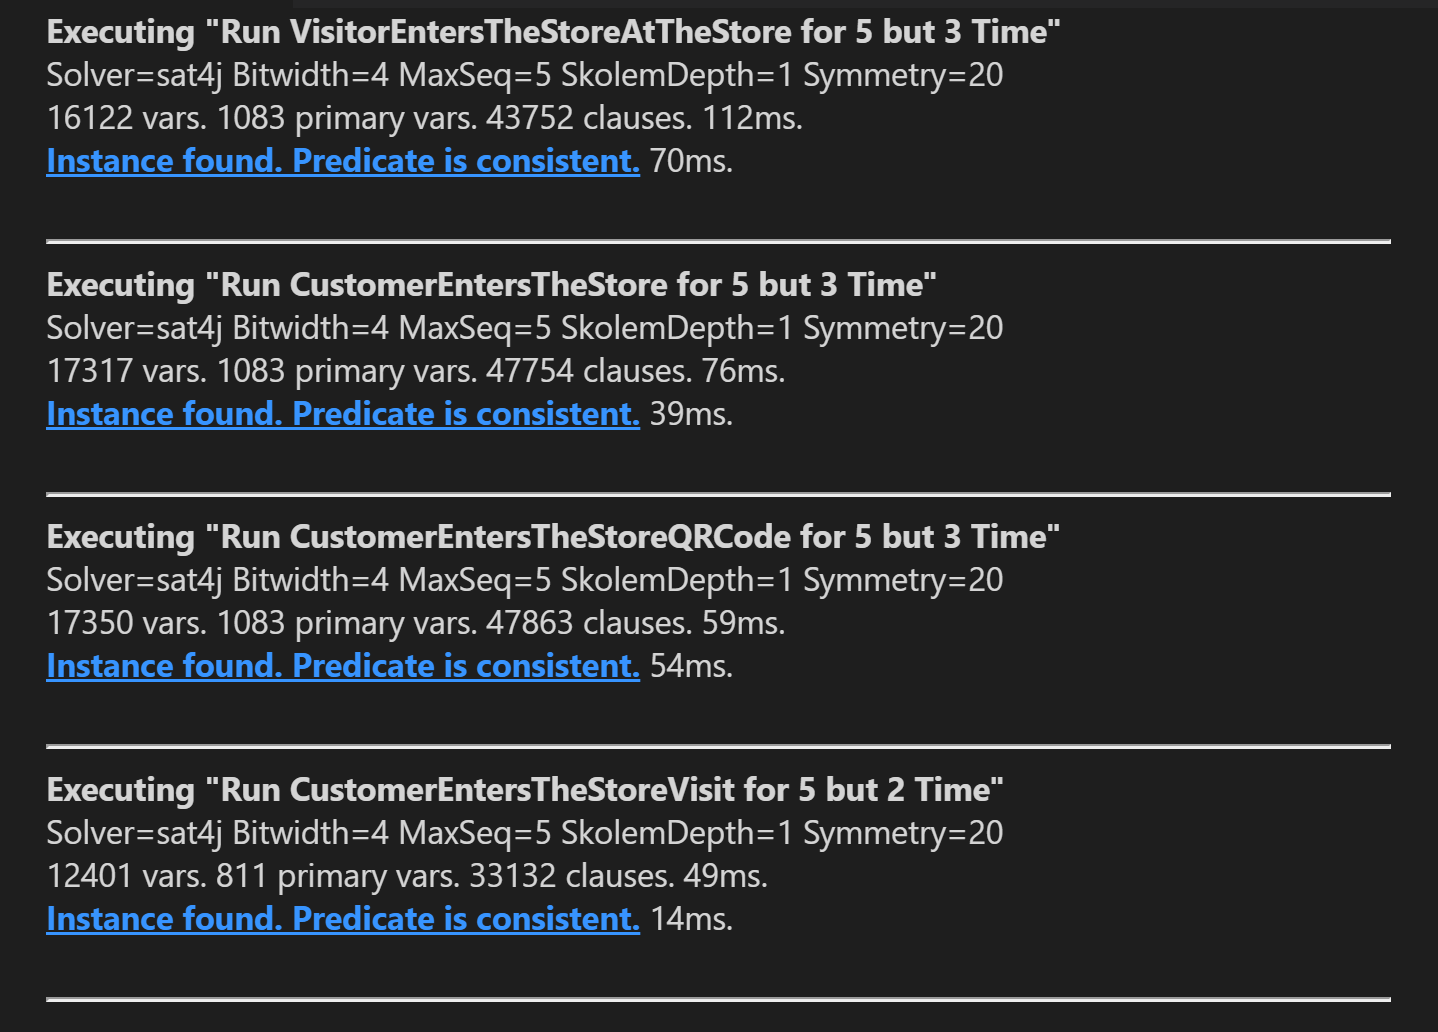
\includegraphics[width=10cm]{proof_of_consistency.png}
    \end{center}

\subsection{Generated world}
Here we include one generated world related to the CustomerEntersTheStoreQRCode pred. The 3 images show the evolution over time of the generated world. We can notice that the Customer is called when the estimatedQueueTime equals the estimatedTravelTime (fig \ref{world2}), that the Entrance is checked through the QRCode and not by an employee and that the realTimeOccupancy increases after the entrance (fig \ref{world3}).  

    \begin{figure}[H]
        \centering
        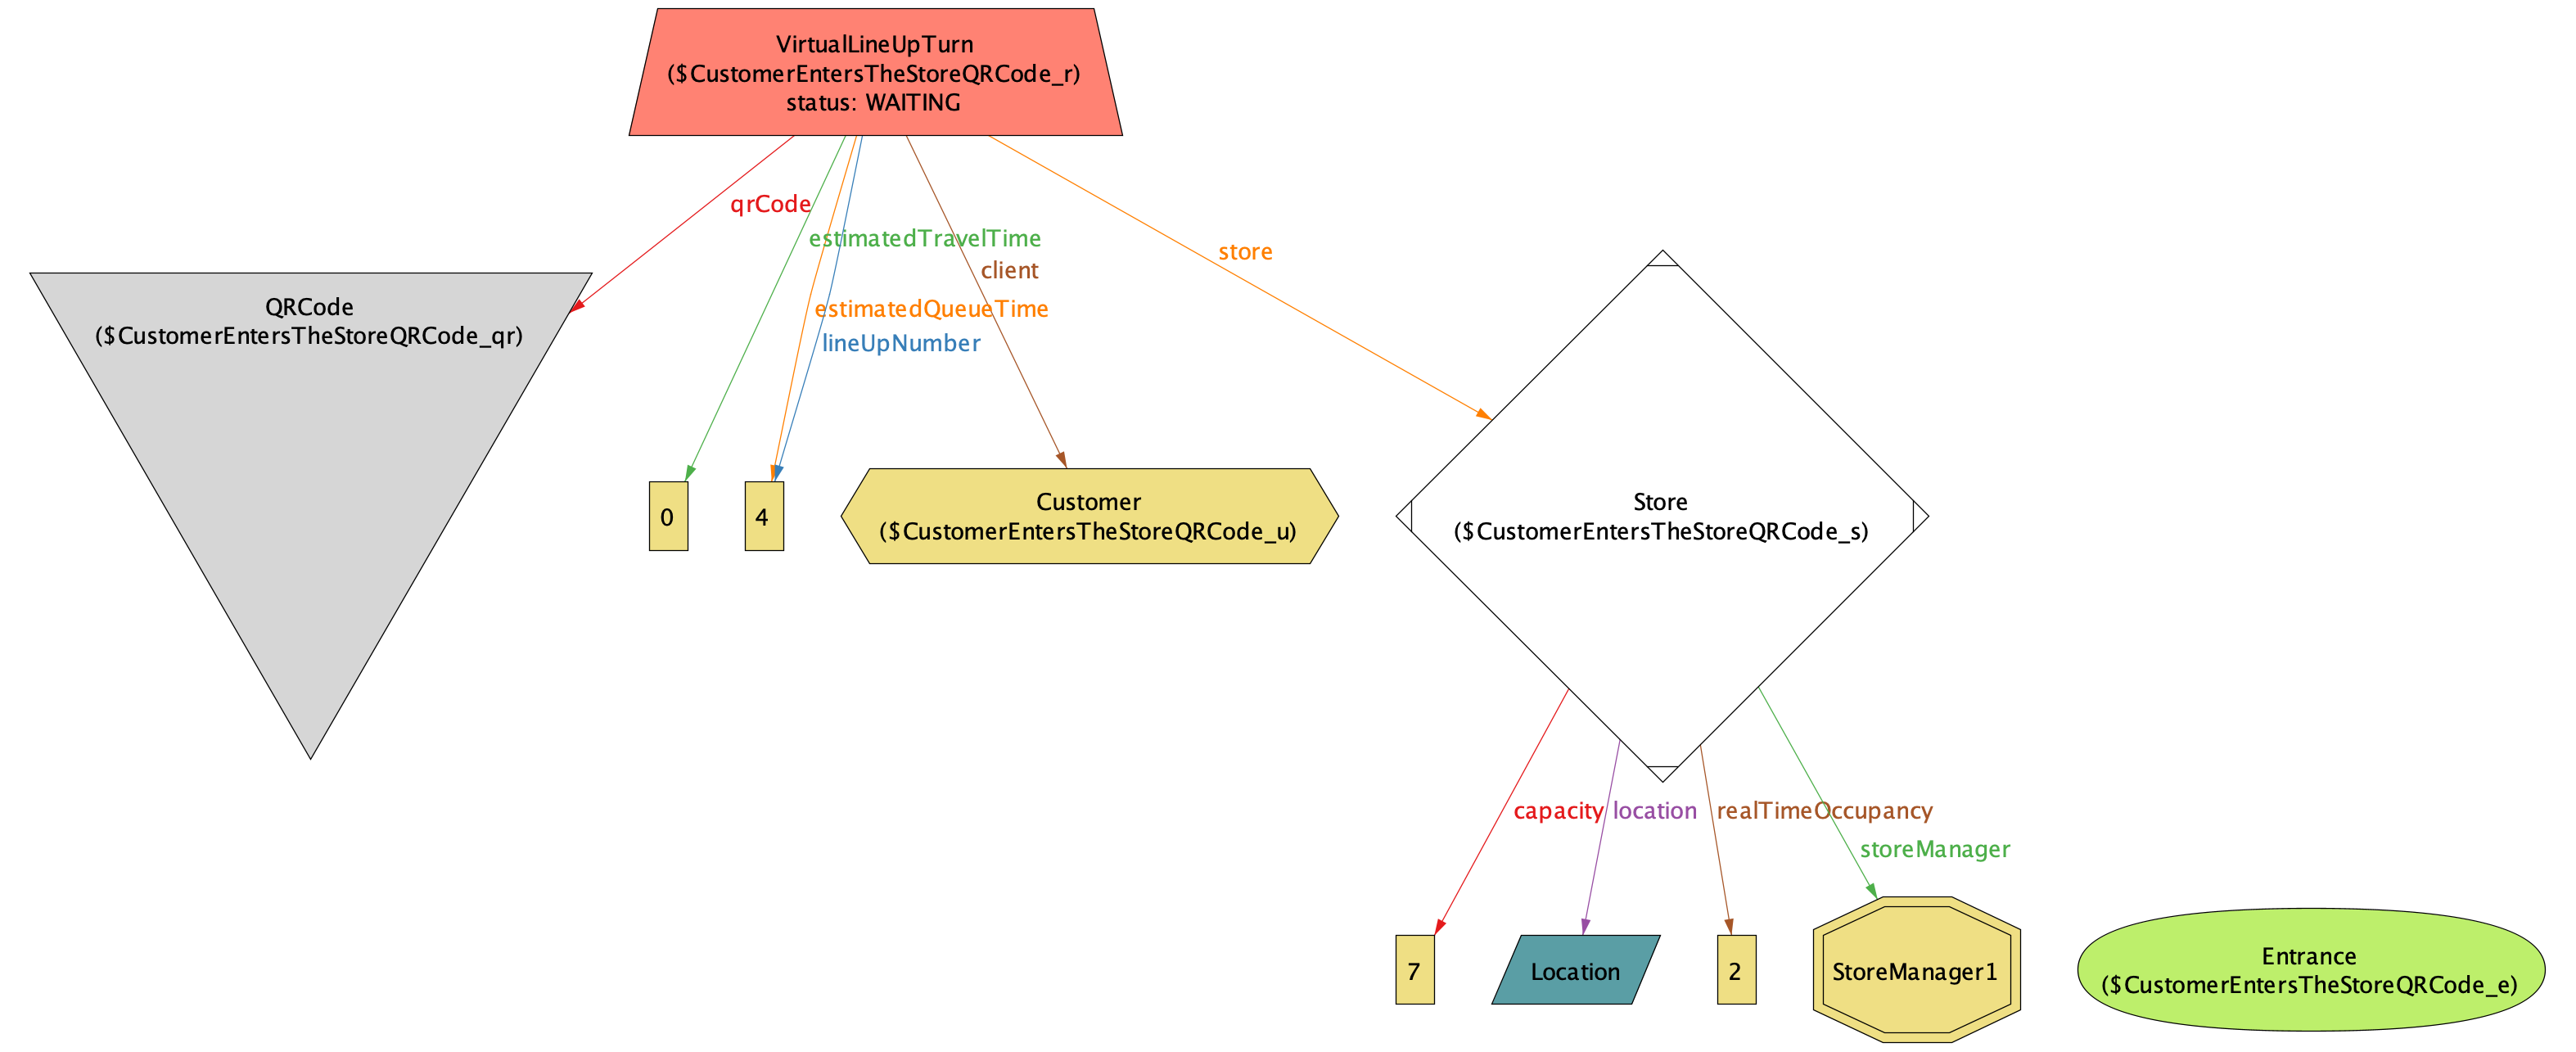
\includegraphics[width=\textwidth]{world1.png}
        \caption{The Customer is waiting in virtual line [Time0]}\label{world1}
    \end{figure}
    \begin{figure}
        \centering
        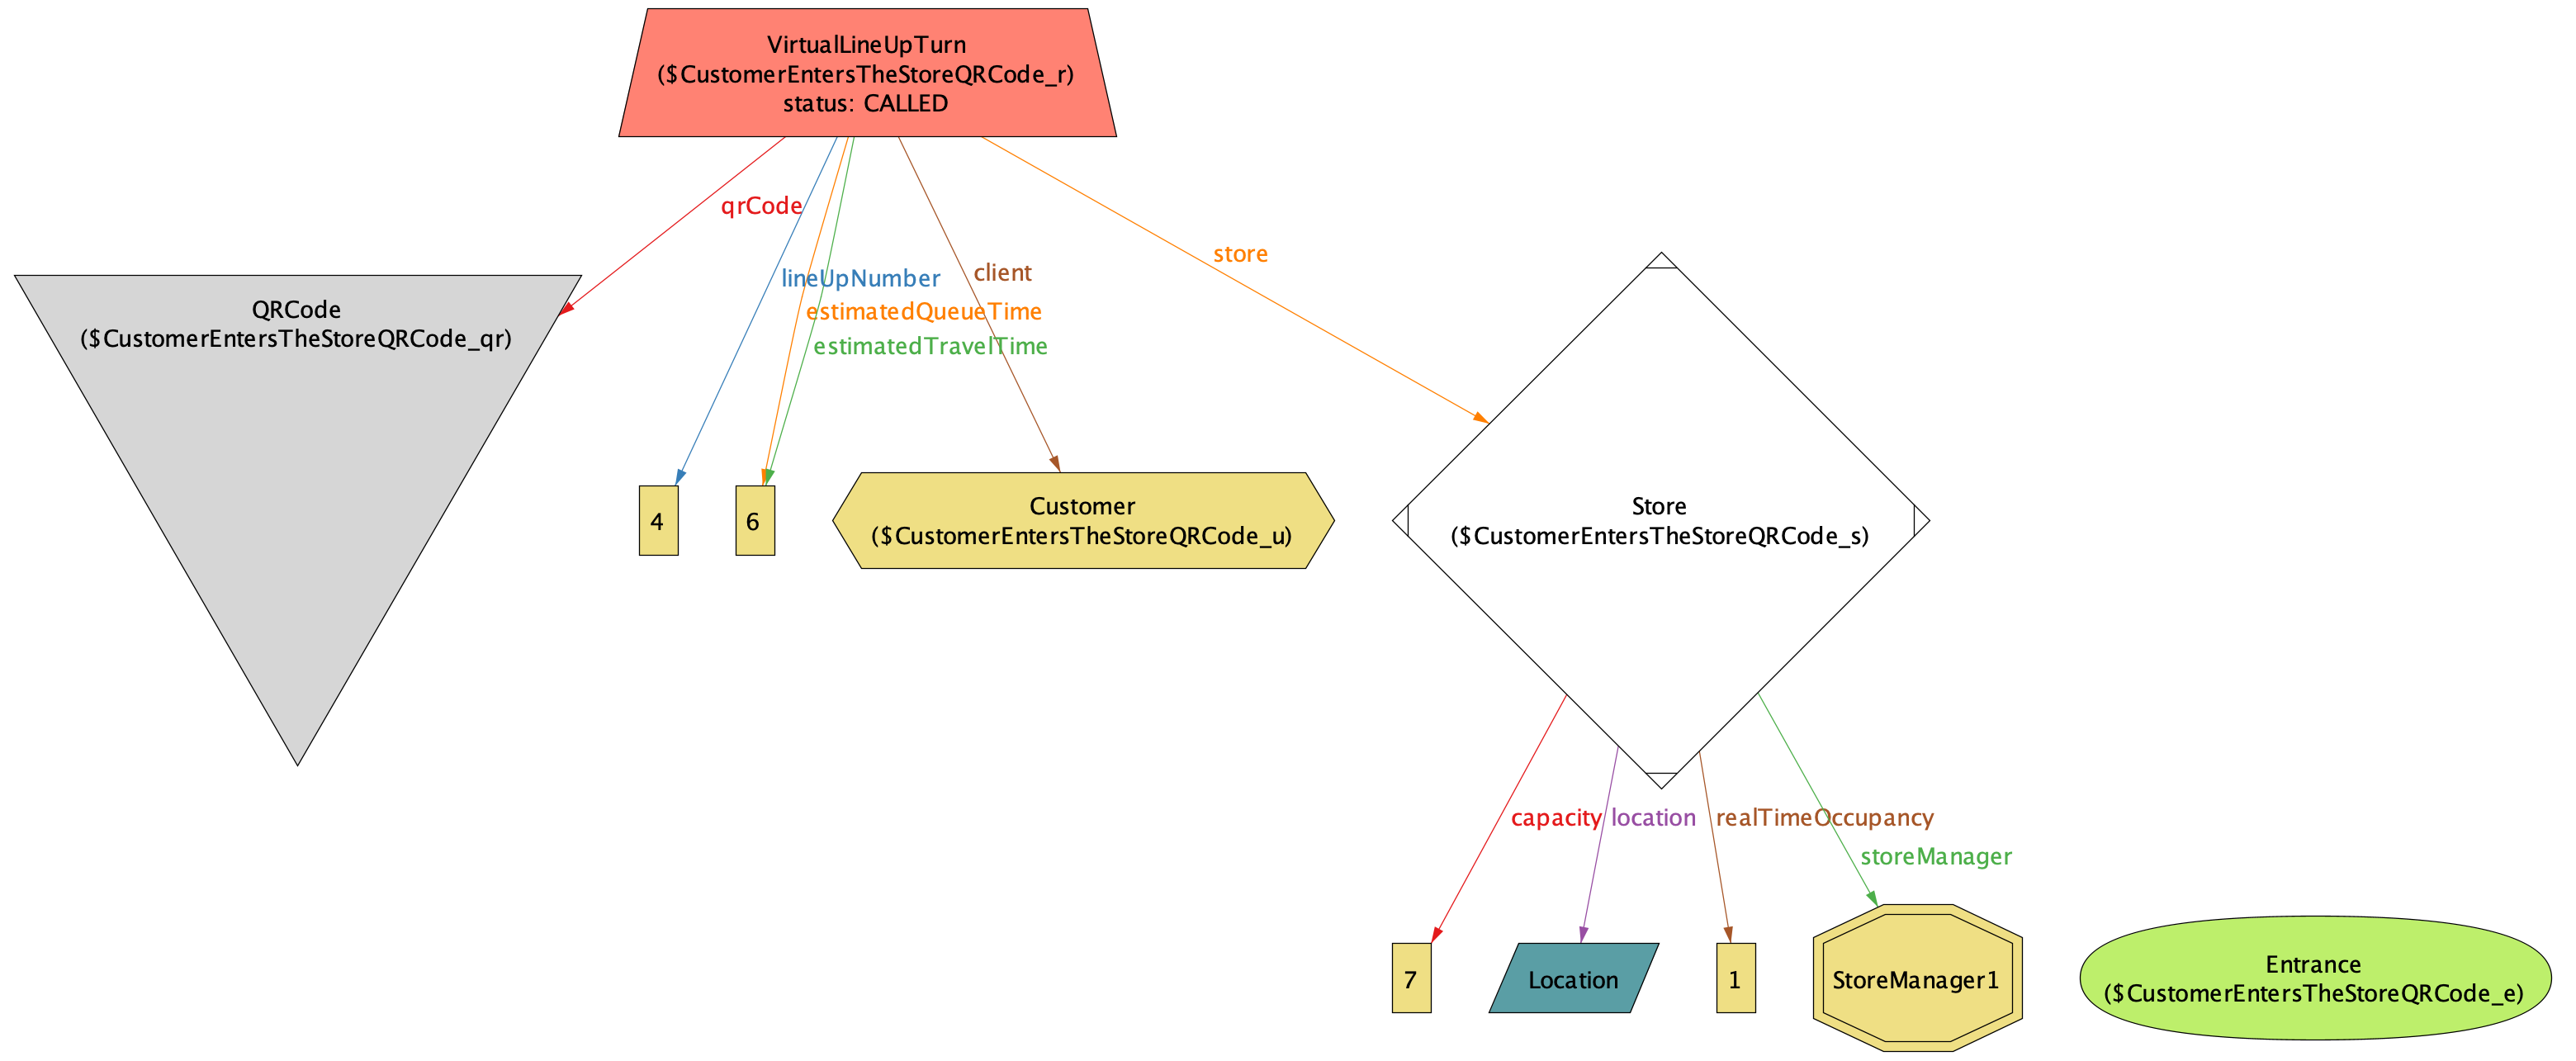
\includegraphics[width=\textwidth]{world2.png}
        \caption{The Customer is called [Time1]}\label{world2}
    \end{figure}
    \begin{figure}
        \centering
        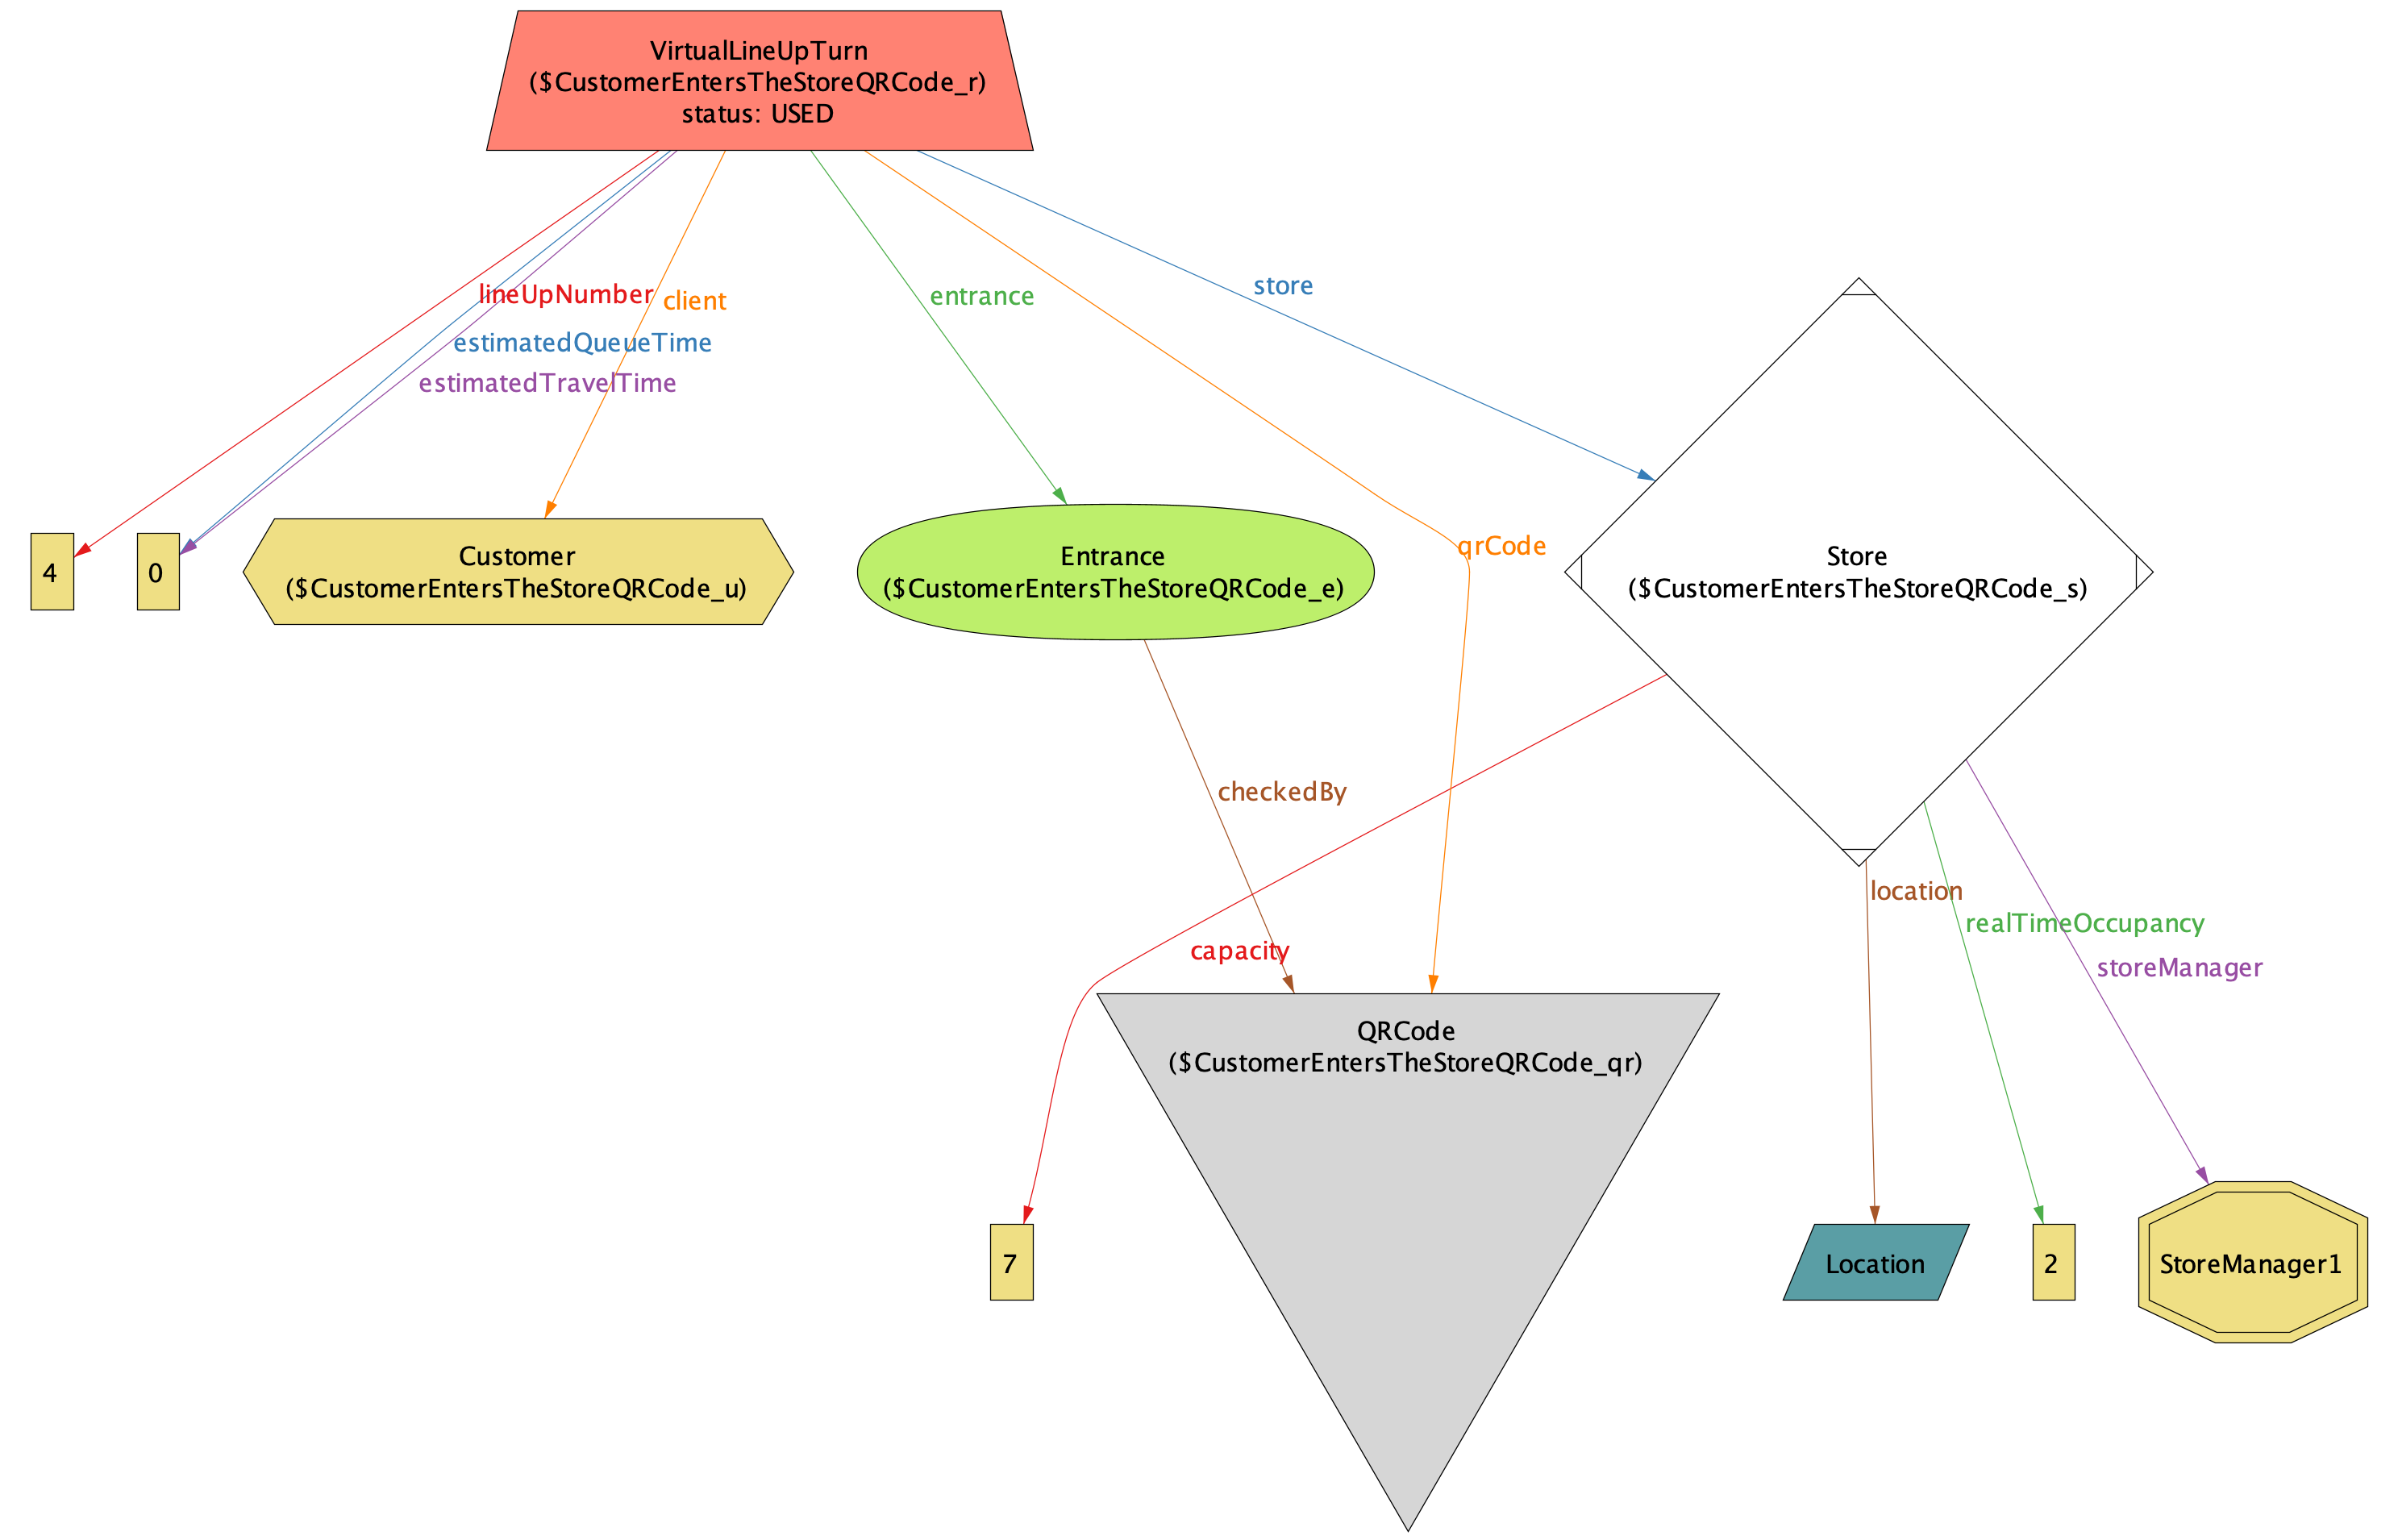
\includegraphics[width=\textwidth]{world3.png}
        \caption{The Customer enters the Store [Time2]}\label{world3}
    \end{figure}